\documentclass[11pt,a4paper]{article}
\usepackage[utf8]{inputenc}\usepackage[T1]{fontenc}\usepackage{lmodern,microtype,parskip}
\usepackage[margin=2cm]{geometry}\usepackage{graphicx,booktabs,tabularx,array,enumitem,xurl,hyperref,fancyhdr}
\hypersetup{colorlinks=true,urlcolor=blue,pdftitle={Pulsar Scout - Database and Machine Learning Integration},pdfauthor={Özcan Öztürk}}
\setlength{\headheight}{14pt}\pagestyle{fancy}\fancyhf{}\fancyhead[L]{\small CMP307 -- Database Management Systems}\fancyhead[R]{\small Pulsar Scout}\fancyfoot[C]{\thepage}
\setlist[itemize]{nosep}\setlist[enumerate]{itemsep=3pt}
\newcolumntype{Y}{>{\raggedright\arraybackslash}X}
\begin{document}
\begin{titlepage}\centering
\vspace*{2cm}{\large Biruni University\\Faculty of Engineering and Natural Sciences}\par
\vspace{1.3cm}{\Large CMP307 -- Database Management Systems}\par
\vspace{1.7cm}{\Huge\bfseries Pulsar Scout}\par\vspace{.5cm}
{\Large Database and Machine Learning Integration\\for Pulsar Candidate Screening}\par
\vspace{1.5cm}{\large Project Report}\par
\vspace{1.3cm}{\Large \"Ozcan \"Ozt\"urk\\Student ID: 230408011}\par
\vfill{25 November 2026}\par
\smallskip\small Implementation, SQL, Dockerfile and editable diagrams accompany this report.
\end{titlepage}

\section*{Abstract}
This project connects a PostgreSQL database to a machine learning pipeline and a small web application. It uses the public HTRU2 benchmark to distinguish labelled pulsar candidates from radio-frequency interference or noise. The source contains 17,898 records and eight numerical measurements. An idempotent INSERT script loads the source into relational tables; the model reads its input directly using SQL rather than reopening a CSV. Three fixed classifiers are compared, and training-only cross-validation selects the model before evaluating a separate 20\% holdout. Membership, metrics and all test predictions are written back in a database transaction, and the browser retrieves the saved records through a Flask API. Random Forest was selected and achieved F1 0.8892, precision 0.8975 and recall 0.8811 on 3,580 test records. A majority-only baseline achieved accuracy 0.9084 but found no positive examples, showing why accuracy alone is insufficient. Query experiments also measured the effect of an index and of serializing feature vectors as JSON. The complete application runs with PostgreSQL and Gunicorn in Docker Compose. This is an educational candidate-screening benchmark, with important limitations for real telescope deployment.

\section{Introduction and Technical Question}
Large candidate lists require a way to prioritize measurements for review. The task here is binary classification using already extracted numeric measurements, not processing telescope images or confirming a new astronomical discovery. HTRU2 labels provide a benchmark for comparing the outputs with known annotations [1,2].

The main technical question is: \textit{Can a reproducible database-to-model-to-database workflow keep source records, experiment splits and predictions linked, while producing useful positive-class classification results?} A second question is how the chosen relational representation and ranking index affect processing time.

PostgreSQL was chosen because typed numeric columns, keys, transactions, views and indexes fit this workflow. These mechanisms are used in applications requiring consistent linked data and auditable results [3]. It also matches the Docker/PostgreSQL setup used in the course. Flask provides a lightweight Python API [6], so the same application can use psycopg for SQL [7] and scikit-learn for modelling.

The prototype is single-user and single-machine. It has no live telescope connection, coordinates, login or external cloud service. Its value is the complete evidence trail through the database, not a claim of scientific novelty.

\newpage
\section{System Architecture and Data Flow}
\begin{center}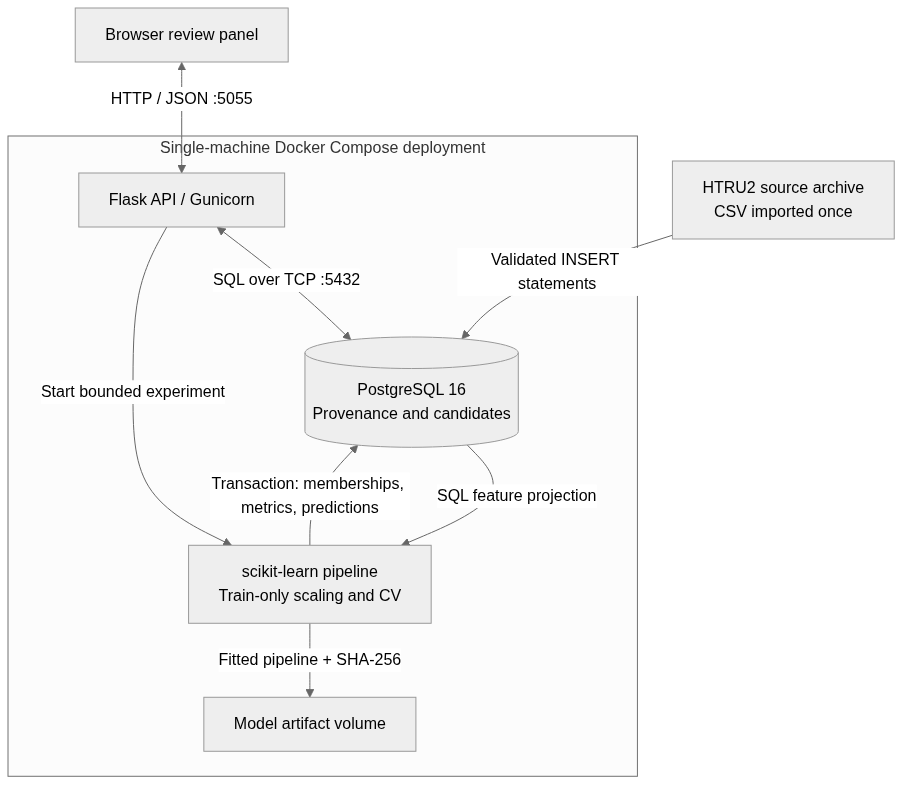
\includegraphics[width=\linewidth,height=12cm,keepaspectratio]{architecture.png}\end{center}
\textbf{Figure 1.} End-to-end architecture. Python modelling is part of the application container, not an independent remote service.

The application and PostgreSQL are separate Compose services on one host [5]. Browser-to-API communication is HTTP/JSON; the app connects to PostgreSQL over TCP port 5432. The host web port defaults to 5055 and can be changed. There is no cache layer or distributed processing.
\begin{enumerate}
\item Load original data using \texttt{sql/02\_seed.sql}. The source version is identified by a SHA-256 checksum and provenance record.
\item Select the eight measurements and target with a parameterized SQL query. Candidate IDs are retained only to link results; neither IDs nor labels enter the feature matrix.
\item Validate the input, split the IDs and run training-only preprocessing and CV. Fit each fixed model and evaluate the held-out records.
\item In a transaction, save split membership, test predictions, metrics and completed status. Save the fitted model separately and record its SHA-256.
\item The API joins saved predictions to source records through the \texttt{prediction\_review} view. The panel supports ranked inspection and false-positive/false-negative filters.
\end{enumerate}
The filesystem model artifact and SQL transaction are separate storage mechanisms. A failed artifact or SQL write marks a run failed; the atomicity claim applies to database result rows, not a distributed transaction across disk and SQL.

\newpage
\section{Database Design}
\begin{center}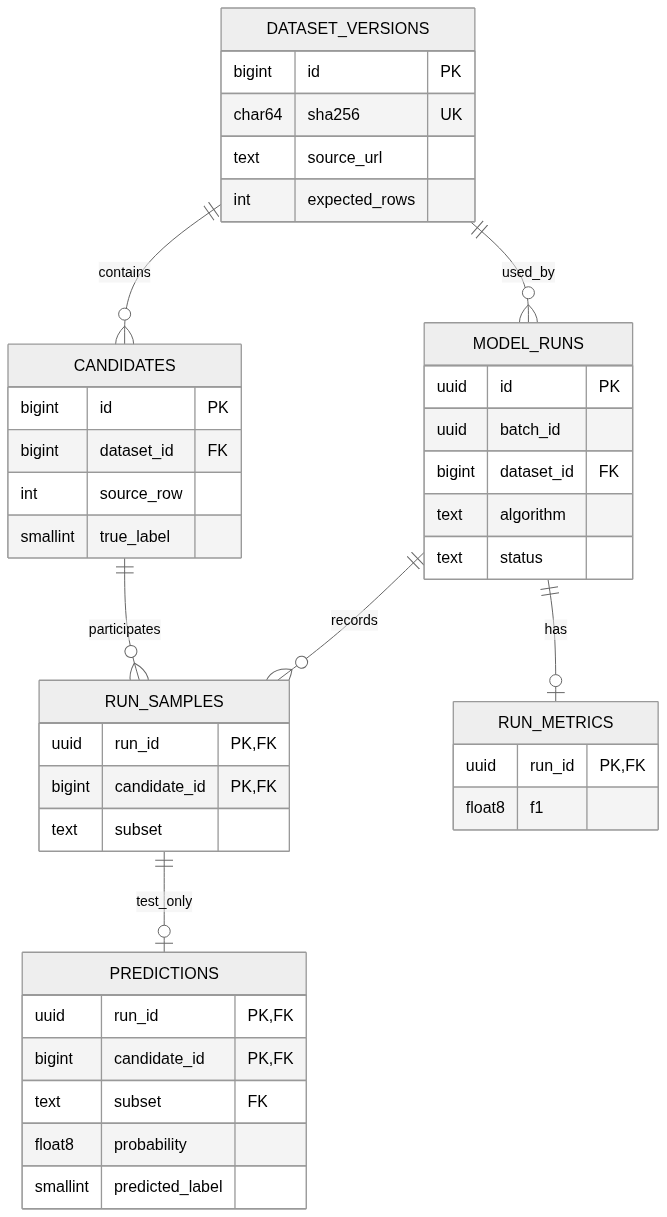
\includegraphics[height=17.5cm,width=\linewidth,keepaspectratio]{schema.png}\end{center}
\textbf{Figure 2.} Relational relationships, keys and selected attributes. The diagram is deliberately compact; the complete types and constraints are in \texttt{sql/01\_schema.sql}. The pair (dataset\_id, source\_row) is unique, rather than source\_row alone. The prediction-to-membership FK also includes subset, which must be test.

\newpage
\subsection{Conceptual Model, Fields and Normalization}
\begin{center}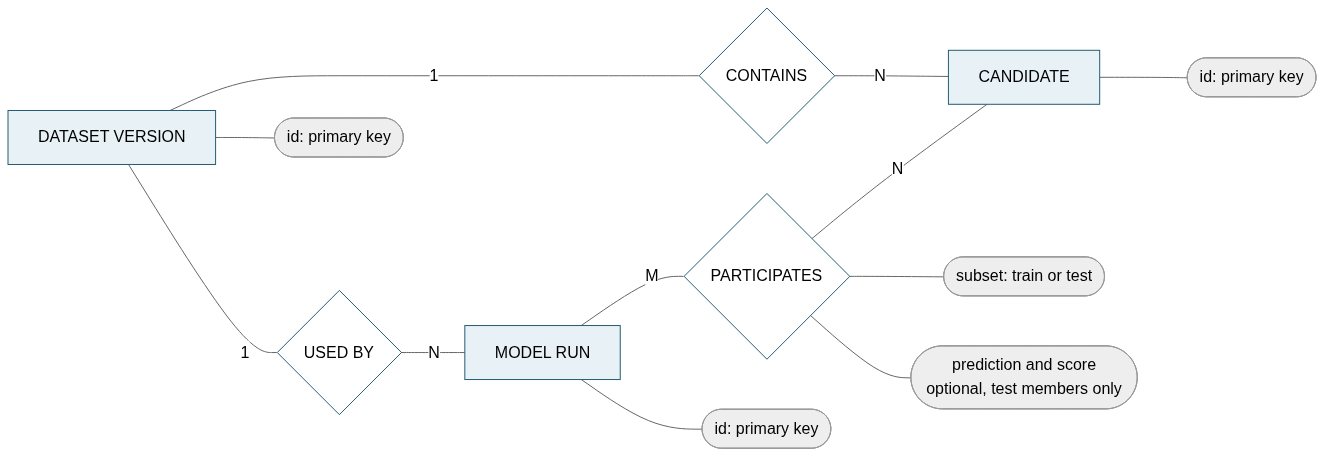
\includegraphics[width=\linewidth,height=5cm,keepaspectratio]{conceptual_er.png}\end{center}
\textbf{Figure 3.} Conceptual Chen-style view. One dataset has many candidates and runs. A run and a candidate participate in an M:N relationship, mapped to run\_samples. Subset is a relationship attribute; only test memberships have prediction records.

\begin{tabularx}{\linewidth}{@{}lY@{}}\toprule
\textbf{Table} & \textbf{Main fields, types and decisions}\\\midrule
 dataset\_versions & BIGINT identity PK; name/source\_url/license TEXT; sha256 CHAR(64) UNIQUE; expected\_rows INTEGER; imported\_at TIMESTAMPTZ.\\
 candidates & BIGINT identity PK and dataset FK; source\_row INTEGER; feature\_1 through feature\_8 DOUBLE PRECISION; true\_label SMALLINT constrained to 0/1.\\
 model\_runs & UUID PK and batch UUID; dataset FK; algorithm/status TEXT; seed BIGINT; split counts INTEGER; threshold/CV F1/timings DOUBLE PRECISION; selected BOOLEAN; parameters JSONB; model SHA and timestamps.\\
 run\_samples & Composite PK (run\_id UUID, candidate\_id BIGINT); subset TEXT constrained to train/test; both IDs are FKs.\\
 run\_metrics & Run UUID is PK/FK; accuracy, precision, recall, F1, ROC-AUC and AP are DOUBLE PRECISION in [0,1]; TN/FP/FN/TP are nonnegative INTEGERs.\\
 predictions & Composite PK (run\_id,candidate\_id); test-only subset; DOUBLE PRECISION score in [0,1]; SMALLINT predicted class 0/1; created\_at TIMESTAMPTZ.\\\bottomrule
\end{tabularx}

Core entity tables keep one value per field and separate source metadata from candidate rows. Run membership resolves M:N without storing lists of IDs in a cell. Dataset metadata depends on dataset ID; measurements depend on candidate ID; membership subset depends on the full run/candidate key. These choices follow the course's 1NF--3NF mapping principles. JSONB holds variable algorithm configuration, not relationships between entities.

Metrics and split counts are deliberate derived audit snapshots. They are not claimed to be redundancy-free source data: tests recompute confusion counts from the saved predictions to check consistency. A trigger additionally checks that a run and candidate belong to the same dataset, which ordinary independent FKs would not establish.

\newpage
\section{Data Preparation and Modelling}
\subsection{Source and Checks}
The source is UCI HTRU2, licensed CC BY 4.0 and attributed to Lyon [1]. It has 16,259 negative examples and 1,639 positives. The ingestion audit checked row width, numeric conversion, finite values and binary labels. No exact duplicate feature vectors were found. Original source bytes, attribution and SHA-256 are supplied with the project.

The source's ARFF attribute names and README prose disagree on the naming order of skewness and kurtosis. To avoid silently changing values, the schema uses positional feature names 1--8 and preserves the original column order. No feature-importance claim requiring that disputed semantic mapping is made. The first and fifth measurements are the profile/DM means; positions two and six are their standard deviations. All values are finite and the two standard deviations are constrained to be nonnegative.

\subsection{Leakage Controls and Model Selection}
A stratified split with random seed 42 reserves 3,580 records for testing and leaves 14,318 for training. The same split is reused across the three fixed algorithms and stored in run\_samples. The source target becomes y only; the eight measurements become X.
\begin{itemize}
\item \textbf{Dummy:} most-frequent class, to expose the imbalance problem.
\item \textbf{Logistic Regression:} StandardScaler plus balanced class weights, maximum 2,000 iterations.
\item \textbf{Random Forest:} 100 trees, minimum leaf size 2, balanced class weights, fixed seed and one modelling thread.
\end{itemize}
Three-fold stratified CV on training records selects the highest mean positive-class F1. The scaler is inside the pipeline and is refitted in each training fold [4]. The test set is not used to select the algorithm or tune the threshold. The predeclared threshold is 0.5. All three fixed models are evaluated once on that holdout for comparison; selection remains the training-CV decision.

No imputation was necessary for this supplied dataset. Scaling is used only for Logistic Regression. No synthetic oversampling or test-set fitting is performed. Scores are not calibrated probabilities.

\subsection{Database Read and Write}
\begin{verbatim}
SELECT id, feature_1, feature_2, feature_3, feature_4,
       feature_5, feature_6, feature_7, feature_8, true_label
FROM candidates WHERE dataset_id = %s ORDER BY id;
\end{verbatim}
This is the model's direct data source. The CSV is used only for the reproducible ingestion script. Each completed model has 3,580 linked prediction rows; a batch of three models has 10,740. The composite membership FK prevents inserting a prediction for a training record. A transaction commits memberships, predictions, metrics and completed status together, with an integration test for rollback after an intentional partial-write failure.

\newpage
\section{Measured Model Results}
The following values were read back from PostgreSQL for the first recorded batch (seed 42). Positive means pulsar. No numbers are illustrative or copied from a paper.
\begin{center}\small
\begin{tabular}{lrrrrrr}\toprule
Model & CV F1 & Accuracy & Precision & Recall & F1 & AP\\\midrule
Dummy & 0.0000 & 0.9084 & 0.0000 & 0.0000 & 0.0000 & 0.0916 \\
LogisticRegression & 0.8434 & 0.9696 & 0.7844 & 0.9207 & 0.8471 & 0.9337 \\
RandomForest & 0.8872 & 0.9799 & 0.8975 & 0.8811 & 0.8892 & 0.9265 \\
\bottomrule\end{tabular}
\end{center}
\begin{center}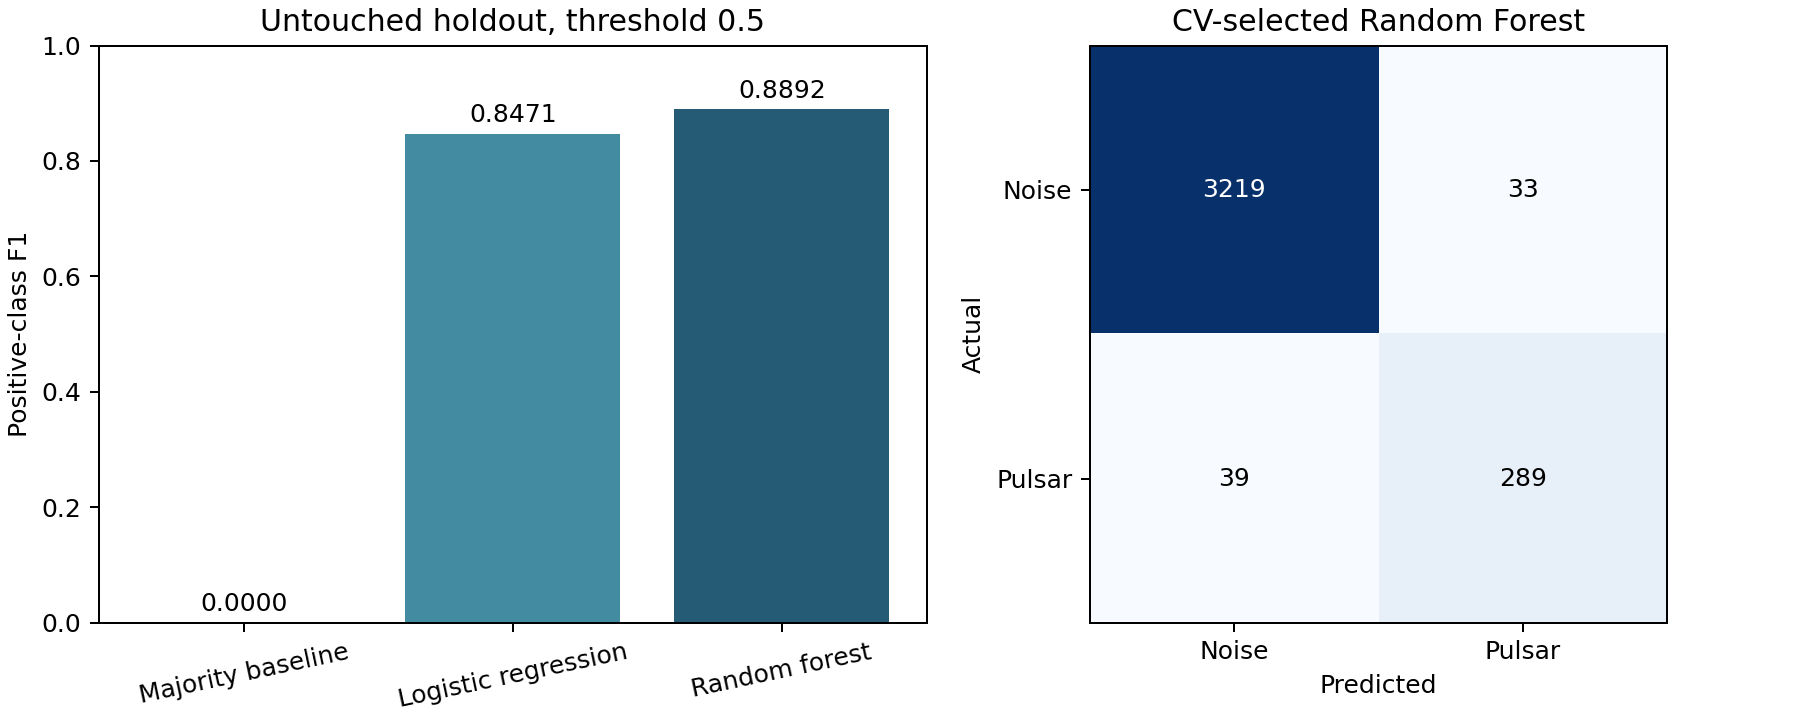
\includegraphics[width=\linewidth]{results.png}\end{center}
\textbf{Figure 4.} Held-out F1 and the selected Random Forest's confusion matrix. Model choice used CV, before this test evaluation.

Random Forest's test counts were TN 3,219, FP 33, FN 39 and TP 289. It found 289 of the 328 positive test cases. The 39 missed positives are an important weakness for a screening application. Logistic Regression had higher recall (0.9207) and ROC-AUC (0.9727), while Random Forest had higher precision and F1. Random Forest's ROC-AUC was 0.9669; being selected by F1 does not mean it wins every metric.

The majority baseline reached accuracy 0.9084 while missing every pulsar. This is why accuracy cannot be the only reported measure. AP means scikit-learn's average precision summary; it is not described as trapezoidal PR-curve area. The baseline AP was the positive-class prevalence, 0.0916.

Local and Docker training reproduced the same reported F1 values with the fixed source, split, parameters and seed. Timing can vary with hardware and concurrent workloads. Repeating the experiment adds history; it does not replace source records. Screenshots can therefore show more than one batch.

\newpage
\section{Data Structure and Query-Time Evaluation}
\subsection{Feature Transport}
The schema keeps the eight values in typed columns rather than a generic attribute/value table. This allows one projection for training and database checks on numeric values. It avoids joins for every feature and does not encode a list of measurements in a text cell.

Two equivalent reads of all 17,898 rows were measured from the same client connection: a normal typed projection and SQL construction of a JSONB array containing the same features. After one warm-up, seven runs were measured per method. Median end-to-end fetch/decoding times were \textbf{59.822 ms} for typed columns and \textbf{224.567 ms} for JSON-array transport.

This comparison includes JSON construction and Python decoding. It does \textbf{not} compare two independently stored physical tables, so it does not establish that every relational design is faster than JSON storage. No feature values were changed and no classification improvement is attributed to representation alone.

\subsection{Ranking Index}
\begin{verbatim}
CREATE INDEX predictions_rank
ON predictions(run_id, probability DESC, candidate_id);

SELECT candidate_id, probability FROM predictions
WHERE run_id = %s
ORDER BY probability DESC, candidate_id LIMIT 20;
\end{verbatim}
Using EXPLAIN (ANALYZE, BUFFERS, FORMAT JSON), the median server execution time over seven warm runs was \textbf{0.027 ms} with the index and \textbf{1.086 ms} without it. The benchmark snapshot contained 10,740 prediction rows. The index was removed only inside a transaction and restored by rollback. Actual plans and all repetitions are in \texttt{docs/evidence\_snapshot.json} [3].

These are small warm-cache, single-machine measurements, not a throughput benchmark. They exclude the browser's rendering time and should not be generalized to other data sizes. The data-structure benefit here is a suitable access path for a specific filter/order workload, together with consistent typed records and traceable relationships.

\subsection{Consistency and Audit Queries}
\begin{verbatim}
SELECT outcome, COUNT(*)
FROM prediction_review WHERE run_id = %s GROUP BY outcome;
\end{verbatim}
This SQL aggregation recomputes the confusion counts from stored results. Tests compare those counts with the metric snapshot, check split sizes and verify that training/test membership does not overlap. Source checksums, run IDs, seeds, parameters and model hashes make the evidence traceable.

\newpage
\section{Implementation, Setup and Verification}
\subsection{Software and Setup}
Tested core versions are PostgreSQL 16.16, Python 3.12, Flask 3.1.3, psycopg 3.3.9, NumPy 2.3.5, scikit-learn 1.8.0 and Gunicorn 27.0.1. Dependencies are declared in requirements files. Start from the supplied repository:
\begin{verbatim}
cp .env.example .env
# Choose a local POSTGRES_PASSWORD in .env.
docker compose up --build -d
docker compose ps
\end{verbatim}
Open localhost:5055, import the dataset and train. Commands also exist as \texttt{python -m pulsar.cli import-data} and \texttt{python -m pulsar.cli train --seed 42} inside the app container. PostgreSQL data and model artifacts use named volumes. Stopping with \texttt{docker compose down} preserves them; adding \texttt{-v} intentionally deletes them. The README gives local Python setup, ports, configuration and query commands.

The managed development proxy required a session CA mounted as a BuildKit secret for pip. TLS verification stayed enabled and that CA was not committed or baked into the image. A local VFS disk limit was resolved by reducing Dockerfile layers. The tracked Dockerfile is intended for normal Docker installations.

\subsection{Verification}
Five integration tests passed, covering source import idempotence and counts, API input/errors, metric recomputation and split integrity, database constraints, and atomic rollback. UI checks passed for stored counts, ranking, FP/FN filters, pagination, source measurement lookup, server-error display and mobile width. No page exceptions were observed. Both database and application containers were exercised, and the full training command ran inside the app container.

The OpenAPI document and Postman collection reproduce API requests. The demonstration recording shows the real application importing, training, writing results and querying them again. It contains explanatory captions; the separate presentation script supports the student's spoken demonstration. No secret is required in the repository.

\subsection{Security and Operational Limits}
The app uses SQL parameters for user values and rejects invalid seeds, UUIDs and filters. The database is bound to loopback on the host. There is no public authentication system: this prototype should remain local or behind an authenticated development preview. A session advisory lock prevents concurrent training jobs, but this is not a distributed worker system. Gunicorn has one worker with threads and an increased timeout for the bounded synchronous experiment.

\newpage
\section{Conclusion and Evaluation}
The project demonstrates the required two-way integration. Source records are first stored in PostgreSQL, features are queried for modelling, and the resulting metrics and predictions return to linked tables. The web panel reads those saved outputs. Its database design, transaction boundaries and validation are part of the application rather than an unused storage layer.

On the recorded holdout, the CV-selected Random Forest obtained F1 0.8892 and correctly identified 289 positive examples, with 33 false alarms and 39 missed positives. The Logistic Regression comparison shows a different recall/precision trade-off. The result is useful as a benchmark demonstration, but missed candidates and uncalibrated scores prevent treating it as an automatic scientific confirmation system.

The source does not include observing-session or physical-object identifiers, so the random record split cannot demonstrate generalization to completely new telescope campaigns. There are no raw signals or coordinates. Real-world evaluation would need independent observation sets, uncertainty/calibration work and an appropriate review policy.

For larger workloads, next steps would include background training jobs, authentication, resource limits, more independent evaluation and a formal benchmark under concurrent load. The existing schema can retain many runs, but no distributed scalability has been measured. Improvement priorities should be chosen from actual workload and scientific needs rather than added only to make the architecture larger.

\section*{References (IEEE)}
\begin{enumerate}[label={[\arabic*]},leftmargin=1cm]
\item R. Lyon, ``HTRU2,'' UCI Machine Learning Repository, 2015. doi: 10.24432/C5DK6R. \url{https://doi.org/10.24432/C5DK6R}
\item R. J. Lyon, B. W. Stappers, S. Cooper, J. M. Brooke, and J. D. Knowles, ``Fifty years of pulsar candidate selection: From simple filters to a new principled real-time classification approach,'' \textit{Monthly Notices of the Royal Astronomical Society}, vol. 459, no. 1, pp. 1104--1123, 2016. doi: 10.1093/mnras/stw656.
\item PostgreSQL Global Development Group, ``PostgreSQL 16 documentation.'' [Online]. Available: \url{https://www.postgresql.org/docs/16/}. [Accessed: Nov. 25, 2026].
\item Scikit-learn developers, ``Common pitfalls and recommended practices.'' [Online]. Available: \url{https://scikit-learn.org/stable/common_pitfalls.html}. [Accessed: Nov. 25, 2026].
\item Docker Inc., ``Docker Compose documentation.'' [Online]. Available: \url{https://docs.docker.com/compose/}. [Accessed: Nov. 25, 2026].
\item Pallets, ``Flask documentation.'' [Online]. Available: \url{https://flask.palletsprojects.com/}. [Accessed: Nov. 25, 2026].
\item Psycopg team, ``Transactions management.'' [Online]. Available: \url{https://www.psycopg.org/psycopg3/docs/basic/transactions.html}. [Accessed: Nov. 25, 2026].
\end{enumerate}
\end{document}
